\documentclass[portrait,final]{baposter}

% Image
\usepackage{graphicx, epsfig, epstopdf}
% Maths
\usepackage{calc, amsmath, amssymb}
% Fonts packages
\usepackage[utf8x]{inputenc}
\usepackage{times, helvet, palatino}

\usepackage{relsize}
\usepackage{bm}

\usepackage{pgfbaselayers}
\pgfdeclarelayer{background}
\pgfdeclarelayer{foreground}
\pgfsetlayers{background,main,foreground}

\graphicspath{{data/}}			% Path to the images
\DeclareGraphicsExtensions{.pdf,.png}	% Figure format


%%%%%%%%%%%%%%%%%%%%%%%%%%%%%%%%%%%%%%%%%%%%%
% Define some personnal commands
%%%%%%%%%%%%%%%%%%%%%%%%%%%%%%%%%%%%%%%%%%%%%
\newcommand{\ie}{\emph{i.e. }}
\newcommand{\eg}{\emph{e.g. }}
\newcommand{\etal}{\emph{et al. }}


\begin{document}
\typeout{Poster Starts}
\background{
  \begin{tikzpicture}[remember picture,overlay]%
    \draw (current page.north west)+(-2em,2em) node[anchor=north west] {\includegraphics[height=1.1\textheight]{silhouettes_background}};
  \end{tikzpicture}%
}

\newlength{\leftimgwidth}
\begin{poster}%
%%%%%%%%%%%%%%%%%%%%%%%%%%%%%%%%%%%%%%%%%%%%%
% Poster Options
%%%%%%%%%%%%%%%%%%%%%%%%%%%%%%%%%%%%%%%%%%%%%
  {
  headerheight=0.175\textheight		% Size of the Title header
  }
%%%%%%%%%%%%%%%%%%%%%%%%%%%%%%%%%%%%%%%%%%%%%
% Title header
%%%%%%%%%%%%%%%%%%%%%%%%%%%%%%%%%%%%%%%%%%%%%
% Eye Catcher
{ \includegraphics[width=0.25\textwidth]{logo/creatis} }
% Title
{\sf
  3D Texture Synthesis for Modeling Realistic Organic Tissues
  \vspace{0.4em}  
}
% Authors
{\sf
\Large
\vspace{.3em}
\coord{Juan-Carlos}{PRIETO}{1,*},
\coord{Chantal}{REVOL-MULLER}{1,*},
\coord{Fran\c coise}{PEYRIN}{1,2,*},
\coord{Patrizia}{CAMELLITI}{3,*},
\coord{Christophe}{ODET}{1,*}
\\
\affil{1}{\begin{small} Universit\'e de Lyon, CREATIS ; CNRS UMR5220 ; Inserm U1044 ; INSA-Lyon ; Universit\'e Lyon 1, France \end{small}} \\ \vspace*{-0.2cm}
\affil{2}{\begin{small} ESRF, BP 220, 38043 Grenoble Cedex, France \end{small}} \\ \vspace*{-0.2cm}
\affil{3}{\begin{small} NHLI, Imperial College London, UK \end{small}} \\ \vspace*{-0.2cm}
\affil{*}{\begin{small} \{prieto, chantal.muller, fran\c coise.peyrin, christophe.odet\}@creatis.insa-lyon.fr, p.camelliti@imperial.ac.uk \end{small}}
}
% University logo
{ \includegraphics[width=0.09\textwidth]{logo/logo_tutelle} }

%%%%%%%%%%%%%%%%%%%%%%%%%%%%%%%%%%%%%%%%%%%%%
% Poster Text
%%%%%%%%%%%%%%%%%%%%%%%%%%%%%%%%%%%%%%%%%%%%%
\headerbox{Introduction}{name=intro,column=0,row=0,span=1}{
Our method derives from Kopf's approach \cite{KFCODLW07}, it starts with a 2D reference image and 
by means of an energy optimization process described by Kwatra \cite{kwatra:2005:SIGGRAPH}, 
it is able to create a 3D texture that resembles the 2D image in every slice. 
It is based in the following equation:
\begin{equation}
 E(o, \{e\} ) = \sum_{t} \sum_{i \in \{x, y, z\}} || o_{t, i} - e_{t, i} ||^r
 \label{equ:imagenergy} 
\end{equation}
The objective is to create models of organs, capable of integrating anatomical, physiological, mechanical and biochemical information.
We model different types of organs and tissues at the cellular level.
The method is divided in two phases, a search phase and an optimization phase.
}

\headerbox{Search Phase}{name=method1,column=0,below=intro,span=1}{
  \hfill
  \begin{minipage}[b]{0.3\linewidth}
	\centering
	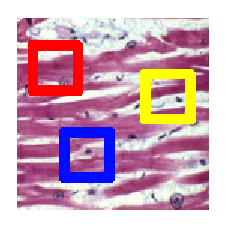
\includegraphics[width=\textwidth]{search_sample}
	(a)
  \end{minipage}
  \hfill
  \begin{minipage}[b]{0.4\linewidth}
	\centering
	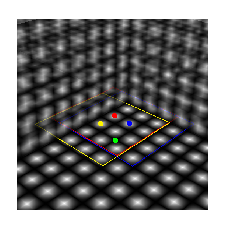
\includegraphics[width=\textwidth]{search_phase}
	(b)
  \end{minipage}
  \hfill
  \MyCaptFig{9x9 Closest neighborhoods (red, blue and yellow squares) found in the sample (a) from the neighborhoods in the volume (b).}
The neighborhoods from the sample and the object are vectorized, for RGB texels we have $9 * 9 * 3 = 243$ values in a single vector. 
Using PCA to reduce the dimensionality of each vector we pass from $243$ to $18$ values approximately.
This enables ANN library to perform a closest neighborhood search, comparing
neighborhoods $x$, $y$, $z$ of a texel $t$ from the object $o$ 
to the sample texture $e$. We seek to minimize equation \ref{equ:imagenergy} by using IRLS (iterative re-weighted least squares). 
This process increases the similarity between the synthetic object and the sample.
  
}

\headerbox{Optimization Phase}{name=method2,column=0,below=method1,span=1}{
The optimization phase consists in averaging the values that affect one texel in the object. 
\begin{equation}
 o_t = \frac{ \sum_{i \in \{x, y, z\}} \sum_{u \in N_i(t)} w_{u, i, t} * e_{u, i, t} }{ \sum_{i \in \{x, y, z\}} \sum_{u \in N_i(t)} w_{u, i, t} }
 \label{equ:texelaverage}
\end{equation}
Equation \ref{equ:texelaverage} shows the value of a texel in the object. 
When the texels present a high variability, clustering is performed to only average those texels that correspond to the principal cluster.
Histogram matching is performed to preserve the global statistics of the object relative to the exemplar \cite{ROLLAND2000} and \cite{Heeger:1995:PTA:218380.218446}.
}

\headerbox{Results}{name=res,column=1,row = 0, span=2}{
The method is able to produce different type of volumetric data from 2D images samples such as 
complex textures provided by digital microscopy of biomedical histological slices.
 
  \begin{minipage}[b]{0.5\linewidth}
	\centering
	\includegraphics[width=0.8\textwidth]{myocyteSg-Ax}\\
	(a)
  \end{minipage}
  \begin{minipage}[b]{0.5\linewidth}
	\centering
	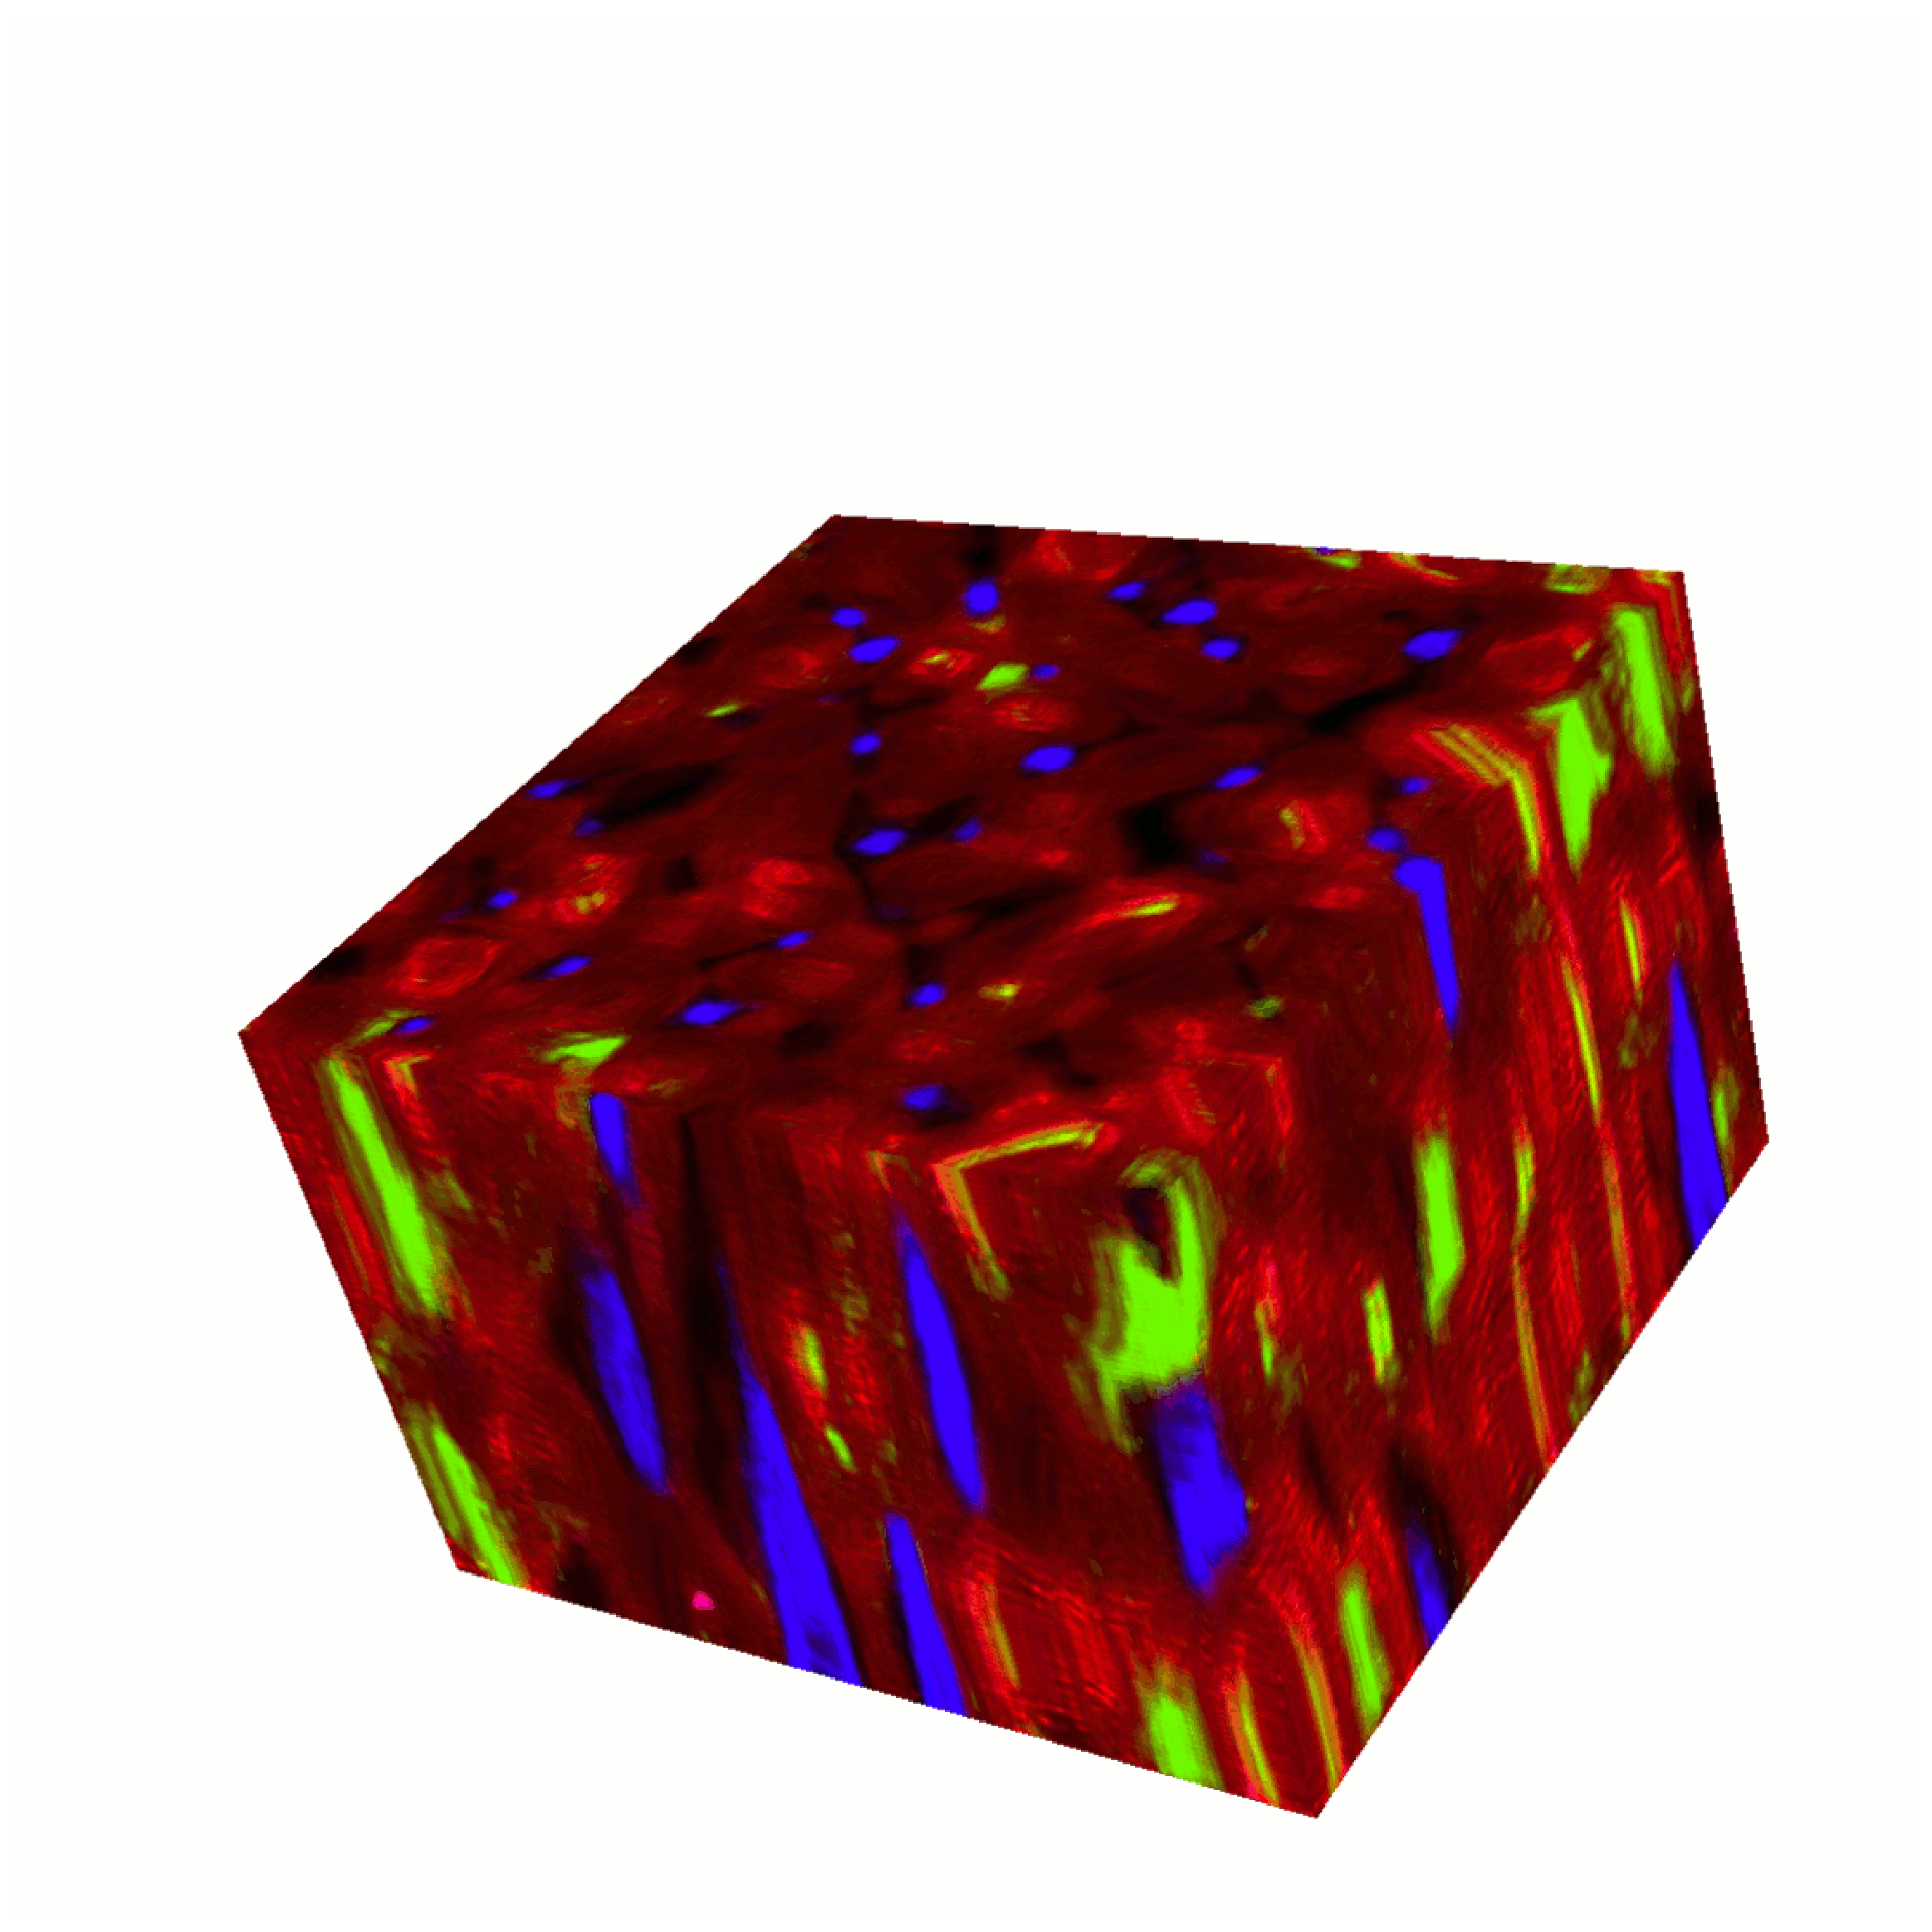
\includegraphics[width=\textwidth]{myocyteAxVol}\\
	(b)
  \end{minipage} \\  
  \begin{minipage}[b]{0.5\linewidth}
	\centering
	\includegraphics[width=0.5\textwidth]{myocyteVol}\\
	(c)
  \end{minipage}  
  \begin{minipage}[b]{0.5\linewidth}
	\centering
	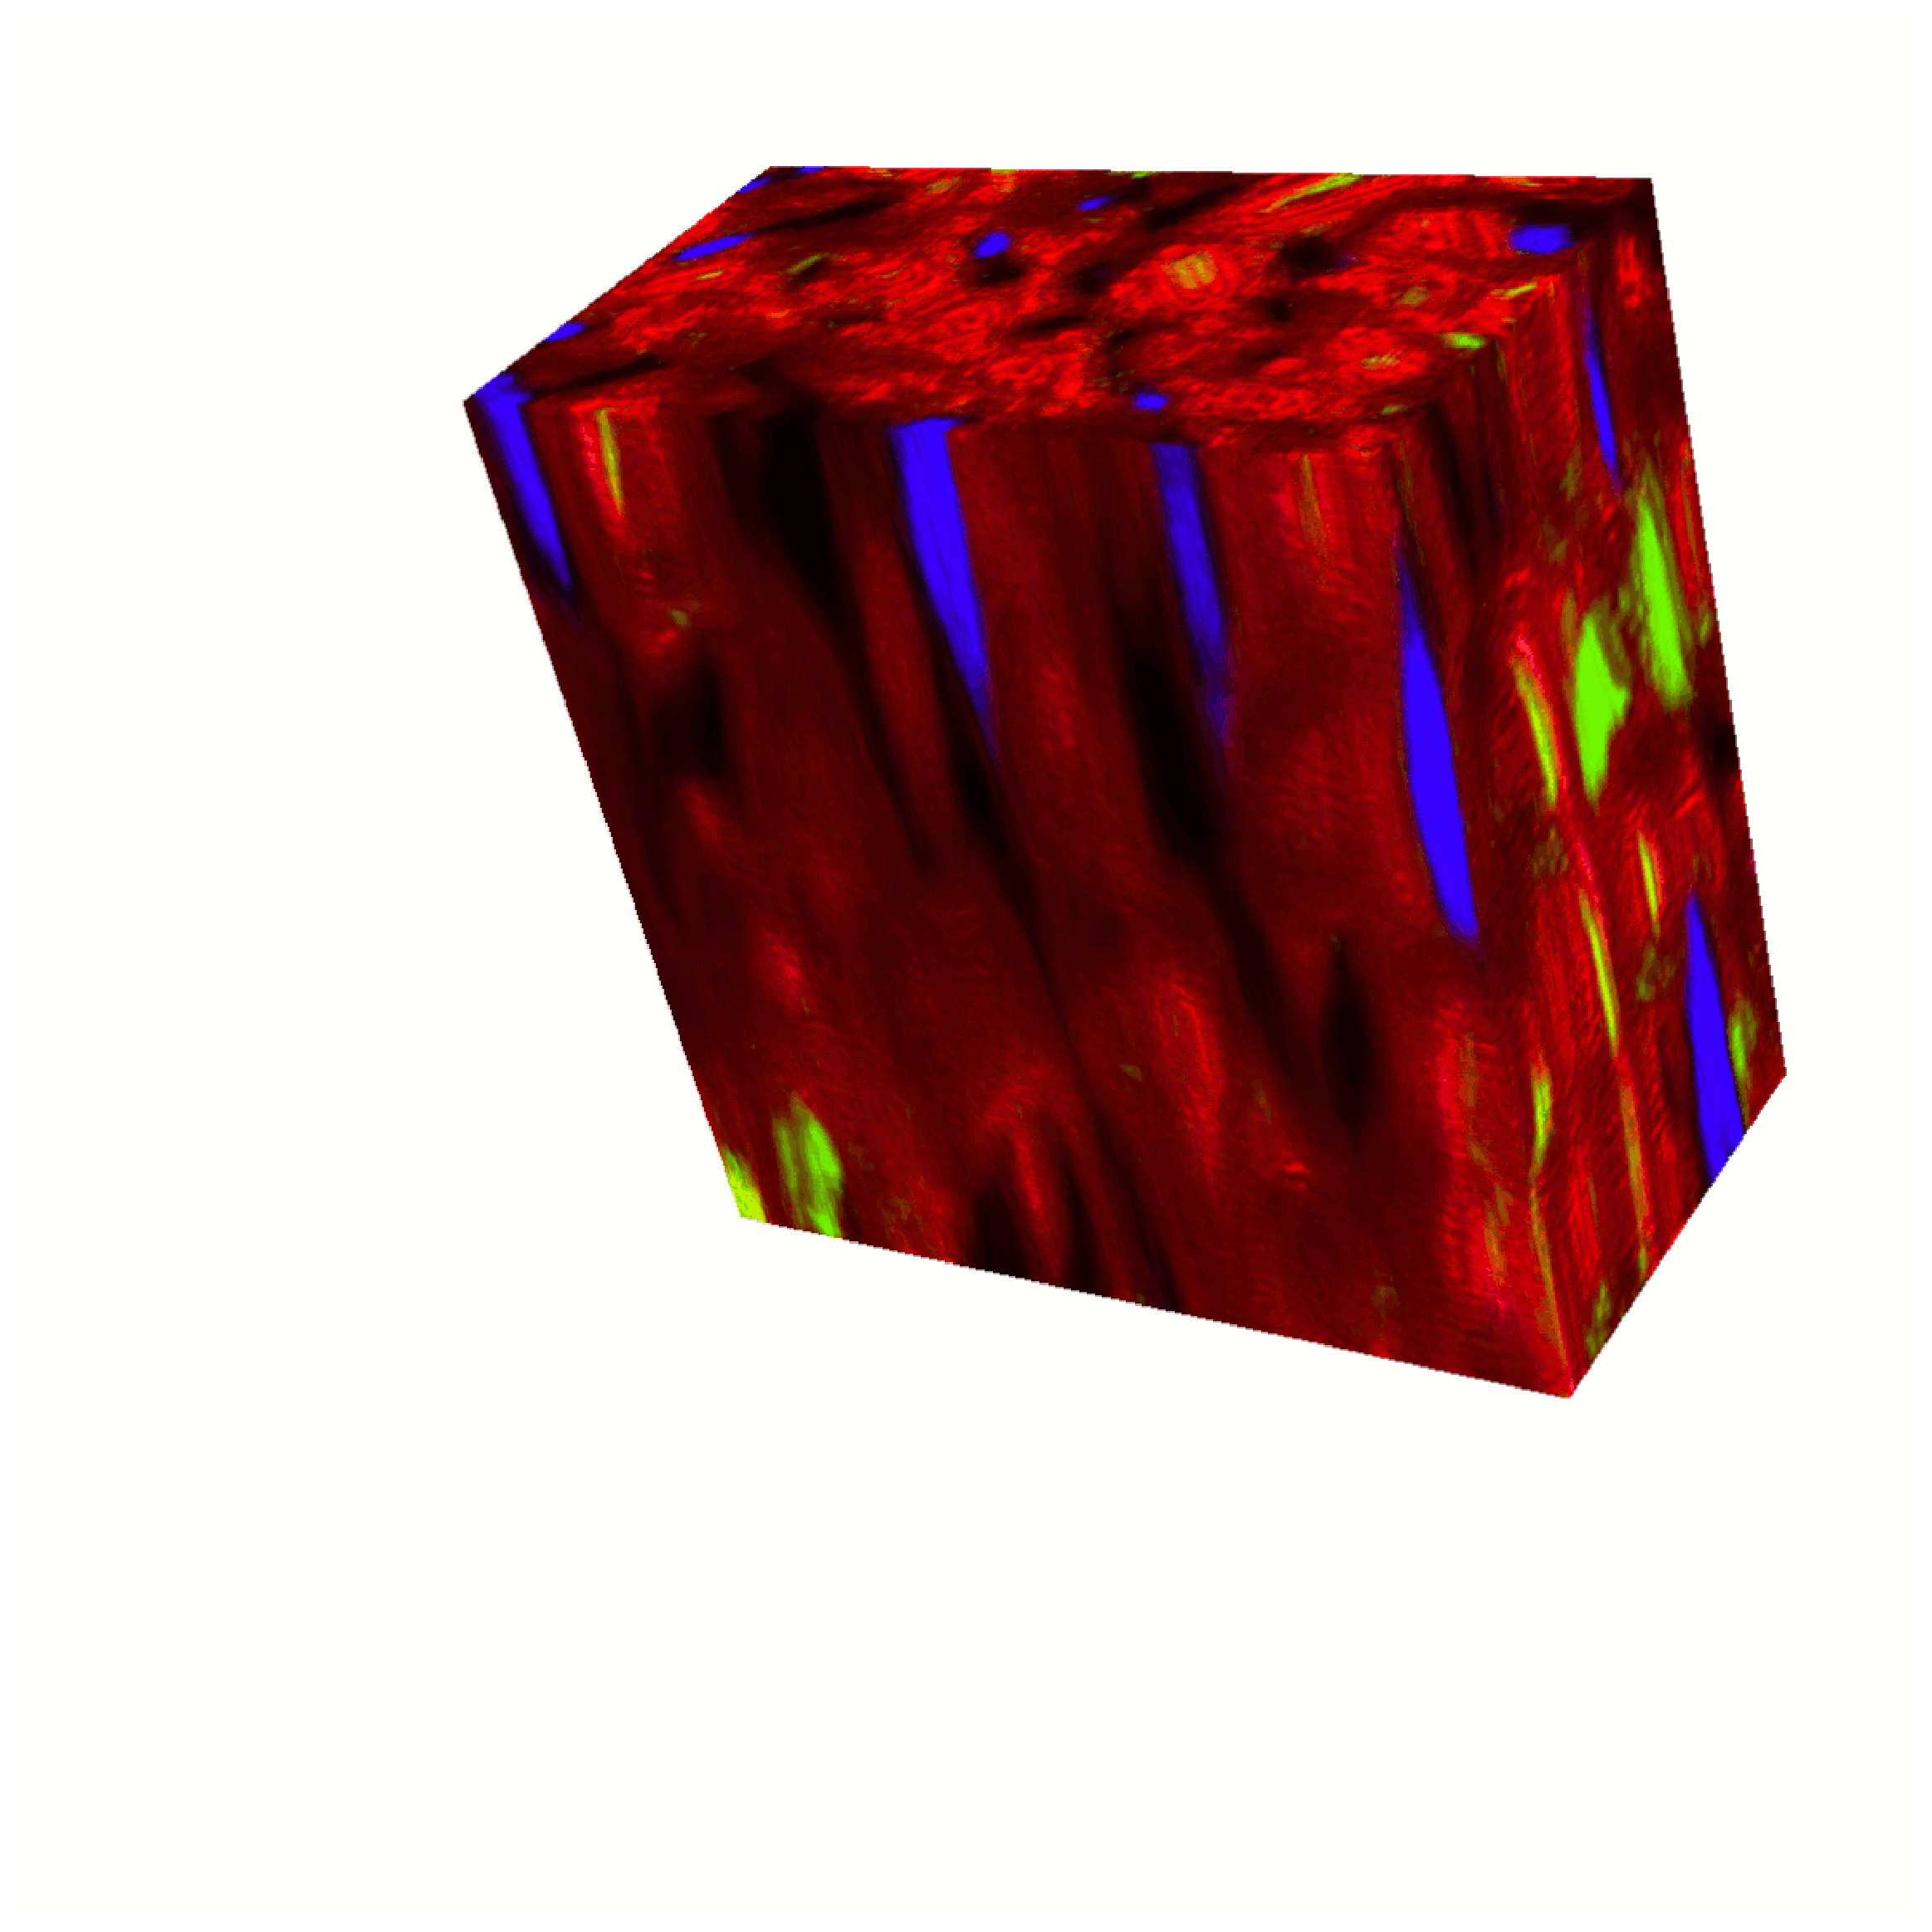
\includegraphics[width=\textwidth]{myocyteSgVol}\\
	(d)
  \end{minipage}
  
  \MyCaptFig{Results of anisotropic synthesis starting from two different textures (a), axial (b) and sagital view (d) of the synthesize volume (c).}
The textured samples were obtained from confocal images, binary masks of the samples are used to calculate the signed distance transform, given as an extra channel to
the optimization process, this is useful to code large textured areas \cite{Lefebvre:2006:ATS:1141911.1141921}.
The 3D texture is representative of cells organisation (myocytes in red and fibroblasts in blue).
The anisotropy of the cells is conspicuous and the contrast of staining is well preserved thanks to the use of the binary masks.
}

\headerbox{Conclusion \& Perspectives}{name=concl,column=1,below=res,span=2}{
Our method allows to create realistic organic tissue from small samples acquired by a digital microscope or
other acquisition devices such as Synchrotron Radiation Computed Micro-Tomography. 
In future work, we will use our method to enhance surface models. We aim to couple the texture synthesis with minimal skeleton 
representations such as the m-reps developed by Pizer \emph{et. al} \cite{Pizer:2003:DMM:945881.945883} we would like to
reproduce the interior of the organs at multi-scale levels using 2D samples of tissue.
}

\headerbox{References}{name=biblio,column=1,below=concl,span=2}{
\renewcommand{\section}[2]{\vskip 0.05em}	% Delete the References at the beginning of the bibliography
\bibliographystyle{amsplain}
\bibliography{3D_Texture_Synthesis_for_Modeling_Realistic_Organic_Tissues}
}

%\headerbox{Acknowledgements}{name=acknow,column=1,below=biblio,span=2}{
%We'd like to thank Chuck Norris \includegraphics[width=0.03\textwidth]{chuck_norris} for his help.
%}

\end{poster}%
\end{document}